\documentclass[12pt]{book}
\usepackage[T1]{fontenc}
\usepackage[utf8]{inputenc}
\usepackage[spanish]{babel}
\usepackage{listings}
\usepackage{float}

\usepackage{graphicx}
\usepackage{color}

\usepackage{amsmath,amssymb}

\usepackage{multicol}
\usepackage{changepage}
\usepackage{cite}
\usepackage{url}
\usepackage[hidelinks]{hyperref}
\usepackage{parskip}

\usepackage{fancyhdr} %para cabeceras


\usepackage[left=2.50cm, right=2.50cm]{geometry}
\lstset{basicstyle=\ttfamily, 
        keywordstyle=\color{blue}, 
        framerule=0pt,frame=single,% fragetMaxme=trBL,frameround=ftttm, 
        lineskip=0pt, 
        emptylines=1, 
        showstringspaces=false, 
        escapechar=·, 
        language=Scala, 
        otherkeywords={toLowerCase, getAs, reduceByKey, sortByKey, first, get, filter getMax, getMin, textFile, SparkSession, splitreplaceAll, map, flatMap, builder, appName, config, getOrCreate, sparkContext, setLogLevel, split, replaceAll, Seq, distinct(), toDF, setCopy, Int, String, mapValues, toDouble, cache, take, option, count, filter, Long, toUpperCase, println, List}
} 

\fancyhf{} 
\renewcommand{\headrulewidth}{0pt} 
\renewcommand{\footrulewidth}{0pt} 
\pagestyle{fancy} 
%\author{Ernesto Villanueva Lazaro}
%\title{Spark}

\begin{document}
%\pagenumbering{Roman}

%

%



 % el titulo con title page y cambiar include por input

\begin{titlepage}


\begin{center}
\thispagestyle{empty}
\vspace*{\baselineskip}
{
\bf\fontsize{19}{0}{\selectfont{INTRODUCCIÓN A APACHE SPARK CON SCALA}}\\[1.5cm]
\bf\fontsize{19}{0}{\selectfont{UNIVERSIDAD COMPLUTENSE DE MADRID}}\\[1.0cm]
\fontsize{11}{0}{GRADO EN MATEMÁTICAS, FACULTAD DE CIENCIAS MATEMÁTICAS}
}

\vspace*{1.5\baselineskip}

{
\bf\fontsize{14}{0}{\selectfont{ERNESTO VILLANUEVA LÁZARO}}
}

\vspace*{0.5\baselineskip}

{
%\bf\fontsize{11}{0}{\selectfont{NOMBRE DEL DEPARTAMENTO AL QUE PERTENECEN}}
}

\vspace*{\baselineskip}

\includegraphics[scale=0.4]{img/ucm.jpg}
\vspace*{3\baselineskip}

{
\bf\fontsize{13}{0}{\selectfont{Trabajo Fin de Grado}}
}

\vspace*{2.5\baselineskip}

{
\hfill\bf\fontsize{14}{0}{\selectfont{Director: Luis Llana}}\\[1.0cm]
%\hfill\bf\fontsize{14}{0}{\selectfont{Tesista: Ernesto Villanueva Lázaro}}
}
\vfill

Madrid, \hfill Julio del 2018

\thispagestyle{empty}

\end{center}

\end{titlepage}

\chapter*{}
%\pagenumbering{Roman}

\section*{Autorización de Difusión}

\begin{center}
Autorización de Difusión\\
\end{center}

ERNESTO VILLANUEVA LÁZARO\\

\begin{center}
Julio de 2018
\end{center}
EL abajo firmante, matriculado en el Grado de Matemáticas de la Facultad de
Ciencias Matemáticas, autoriza a la Universidad Complutense de Madrid (UCM) a difundir y
utilizar con fines académicos, no comerciales y mencionando expresamente a su autor, tanto  el presente Trabajo Fin de Grado: “Introducción a Apache Spark con Scala.” y el código, realizado durante el curso académico 2017-2018 bajo la dirección de Luis Fernando Llana Díaz con el objeto de incrementar la difusión, uso e impacto del trabajo en Internet y garantizar su preservación y acceso a largo plazo.\\


\textbf{Fdo.}

\begin{center}
Ernesto Villanueva Lázaro

\end{center}

\cleardoublepage
\pagenumbering{Roman}
\renewcommand{\contentsname}{Índice}
\tableofcontents
\thispagestyle{empty}
\begin{titlepage}
\null
\vfill
\begin{center}
\textbf{Agradecimientos}\\
\end{center}


A mi familia, por todo su apoyo. \\

A María, por su ayuda y consejo.\\

A Stratio, por la formación que recibí al iniciar mi vida laboral, en especial, a Jorge López Malla,  por animarme a resolver ejercicios, incluidos en esta memoria, de registros de vuelos en EEUU a partir de un dataset público.\\

\vfill\null

\end{titlepage}

\thispagestyle{empty}



\chapter*{}
%\thispagestyle{plain}


\section*{Resumen}
\leftmark{} 
\rightmark{} 

Estamos generando más datos que nunca: según \textit{World Wide Web Size} \cite{wwws}, se llegó a alcanzar en el 2016 la cifra de un Zettabyte, o, lo que es lo mismo, 1.099.511.627.776 GB. En 2017, durante cada minuto se realizaron más de 3.8 millones de búsquedas en Google, se escucharon más de 1.5 millones de canciones en Spotify, se enviaron más de 29 millones de mensajes por whatsapp, 400 horas de video se subieron a Youtube… Frente a estas cifras, el uso de las herramientas tradicionales no resulta el más apropiado para abordar análisis de datos.\\

Cuando la cantidad de información es demasiado grande para ser tratada en una sola máquina, ha de paralelizarse. Spark es un framework de procesamiento distribuido en memoria que hace uso del paradigma de programación MapReduce para realizar computación distribuida en un clúster. En esta memoria nos familiarizaremos con esta herramienta, aprenderemos cómo trabajar con Spark y cómo Spark opera. 



{\setlength{\parskip}{30mm}
\section*{Palabras clave}
}
Spark, Big Data, dato, scala, hadoop, Apache, clúster, RDD, Dataset, 
DataFrames, Shuffle

\chapter*{}

\section*{Abstract}

resumen en ingles


\section*{Keywords}
Spark, Big data, scala, hadoop, Apache, clúster, RDD, Dataset, DataFrames, Shuffle


\chapter{Introducción}
\pagenumbering{arabic}

La Historia siempre ha tomado como referencia acontecimientos de vital importancia que han introducido cambios fundamentales en la historia de la humanidad;  podemos encontrar activos que sobresalen con respecto al resto, algunos tan relevantes para su época que incluso los bautizan: Edad de Piedra, Edad del Bronce, Edad del Hierro. Más recientemente podemos encontrar el carbón, o tras él el petróleo, pero si tuviéramos que destacar  unos elementos actuales por encima de otros para señalarlos como el epicentro de nuestra sociedad, serían los datos, fuente de la información, y, por tanto, del poder.\\

En la economía digital actual los datos constituyen el activo más valioso de muchas empresas. Nos estamos adentrando en la era del Big Data, prueba de esto es que hasta 1.2 ZB de datos IP circularon a través de Internet en 2016 \cite{0cisco} o el crecimiento sin precedentes en la velocidad a la que son producidos; en los últimos dos años se ha creado el 90 por ciento de los datos que hay en el mundo \cite{0IBM}. \\

En este contexto surgen nuevos términos , como “huella digital”, empleado para referirnos al rastro que dejamos al navegar e interactuar con la red, que abarca desde qué páginas visitamos, a cuánto tiempo pasamos en ellas y dónde clicamos, nuevas empresas, o alguna ya existente, que han sabido aprovechar la importancia del dato, como Amazon, Netflix, Facebook o Google, nuevas leyes \cite{0RGPD} que actualizan las ya existentes para adecuarlas al nuevo contexto, nuevas profesiones dedicadas a explotar y aprovechar el valor del dato, como los \textit{Data Scientist} y los \textit{Data Developer}, así como multitud de herramientas con las que hacerlo, como Hadoop Mapreduce, Apache HBase, Apache Hive, Apache Kafka, Apache Mesos, Apache Pig... \\

En esta memoria vamos a introducirnos en el framework Apache Spark, herramienta que , como veremos, nos permite manejar grandes cantidades de información de manera rápida y versátil, ofreciéndonos la posibilidad de trabajar con datos estructurados, semi-estructurados o no estructurados, capaz de tratar con multitud de formatos como CSV, JSON, procesar datos en streaming, aplicar machine learning sobre nuestra información o hacer estudios sobre grafos y, además, podremos hacer esto en diferentes lenguajes. La manera que hemos encontrado más adecuada de trabajar con Spark es a través de su lenguaje nativo Scala, y que en los últimos años se ha convertido en el lenguaje basado en JVM más popular tras Java \cite{0PYPL}. \\

Para ello,  partiremos desde cero, estudiando los conceptos clave para entender cómo trabaja Spark y finalizaremos con unos ejemplos donde poder poner en práctica lo aprendido. En el transcurso de esta memoria nos apoyaremos  especialmente en dos libros de referencia, Spark the Definitive Guide \cite{stdg} y High Perfomance Spark\cite{HPerfomance}, entre otros muchos.\\

Aunque Spark fue diseñado pensando en ser usado sobre un clúster, para la realización de este trabajo se ha utilizado un ordenador personal.\\


\section{Metodología}

El trabajo se va a realizar en cuatro fases:

En la primera, presentaremos a Spark, haremos un repaso sobre su historia, los motivos que llevaron a su creación  y estudiaremos los componentes que configuran el ecosistema Spark.

En la segunda, estudiaremos las abstracciones que usa Spark para manejar datos, cómo operar sobre ellas y empezaremos a entender el impacto que tiene la manera de organizar nuestro código en Spark.

En tercer lugar, vamos a estudiar qué sucede cuando se ejecuta código en Spark, cómo se organizan sus distintos elementos en un clúster y la manera que tiene de transformar el código de un usuario en un trabajo realizado.

Acabaremos poniendo algunos conceptos en práctica mediante el estudio de vuelos realizados en EEUU.

\chapter{¿Qué es Spark?}
\fancyhead[RE,LO]{\leftmark} 
\fancyhead[LE,RO]{\rightmark} 
\fancyfoot[CE,CO]{\thepage} 
Responder a esta pregunta sin divagaciones es posible: Apache Spark es un motor de código abierto de computación en memoria unificado, con un conjunto de bibliotecas para el procesamiento paralelo de datos en clústeres de computadoras. Sin embargo, no sería lícito para su entramado significativo que no nos adentrásemos en tal definición, pues Spark  posee varias características  relevantes para el mundo de la computación.\\

Veamos algunas de sus propiedades:\\

\begin{itemize}
\item Es compatible con Python, Java, R y Scala, su lenguaje nativo.\\

\item Utiliza commodity hardware, lo que supone que pueda ser utilizado desde en un ordenador portátil a en clúster de miles de servidores, pues no requiere de computadores avanzados para su utilización.\\

\item Tiene la capacidad de realizar la mayoría de las operaciones en memoria (sin necesidad de escribir a disco). Por esta razón, podemos afirmar que está dotado de mayor rapidez de la que tienen otras opciones, como Hadoop Map Reduce.\\

\item Ofrece una plataforma unificada que admite una amplia gama de tareas para el análisis de datos, como la carga de datos en crudo, las consultas SQL, el machine learning, el cómputo en streaming o el tratamiento de grafos, todo esto a través del mismo motor de computación y con un conjunto consistente de APIs. \\

\item La filosofía que persigue Spark con esta visión unificada es la de la combinación de diferentes tipos de bibliotecas y procesamientos dispares, tal y como viene exigiendo el mundo real. Referente a las bibliotecas, cabe decir que además de las bibliotecas estándares, de las que hablamos en el siguiente punto, Spark también admite bibliotecas externas publicadas por las comunidades de código abierto.\\

\item Las bibliotecas estándares de Spark, son la mayor parte del proyecto de código abierto. Pese a que las bibliotecas han crecido para ampliar su funcionalidad, el motor central Spark (Sparkcore) apenas se ha modificado desde la fecha de su lanzamiento.\\

\item Su estructura homogénea permite realizar análisis de manera más simple y más eficiente.\\

\item Es importante señalar que Spark, como motor de computación, no tiene como fin almacenar datos, sino manejar la carga de datos de sistemas de almacenamiento y la realización de cálculos.\\

\item Puede ser utilizado en una gran variedad de sistemas de almacenamiento persistentes, incluidos sistemas de archivos distribuidos, como Hadoop HDFS, buses de mensajes, como Apache Kafka, o sistemas de almacenamiento en la nube, como Azure Storage o Amazon S3.\\

\end{itemize}

\chapter{Breve Historia sobre Spark}

Spark surge, en primera instancia,  en la universidad UC Berkeley en 2009 como proyecto de investigación doctoral de Matei Zaharia dirigido por Ion Stoica. Por aquel entonces, Hadoop MapReduce era el motor de programación paralela dominante. Un año más tarde se publicó un artículo titulado “Spark: Cluster Computing with Working Sets”, por Matei Zaharia, Mosharaf Chowdhury, Michael J. Franklin, Scott Shenker e Ion Stoica. \cite{learnSpark}\\

El objetivo perseguido con la creación de Spark era suplir aquellos casos de uso en los que MapReduce resultaba ineficiente. Para ello, trabajaron con usuarios de Hadoop MapReduce con el fin de detectar los puntos fuertes y débiles de esta tecnología, llegando a la conclusión de que debían mejorar los procesos iterativos, aquellos en los que se requieren múltiples pases para procesar los datos y aquellos procesos que requieren una gran cantidad de consultas.\\

Para solventar estos problemas, Spark se basó en la programación funcional, diseñando de este modo una API sobre un nuevo motor, capaz de realizar cálculos en memoria sobre los datos.
Tras esto, su siguiente objetivo fue crear un conjunto de bibliotecas a través de las cuales se pudieran escribir aplicaciones big data con diferentes enfoques usando el mismo framework. Así nacieron MLib, GraphX y Spark Streaming.\\

En 2013 el proyecto se donó a la Apache Software Foundation. En ese mismo año, Matei Zaharia, Ion Stoica, Ali Godsi, Reynold Xin, Patrick Wendell, Andy Konwiski y Scot Shenker fundaron Databriks, empresa con la que fortalecer el proyecto. Al año siguiente, Databricks obtuvo un nuevo récord mundial en la ordenación a gran escala usando Spark. Actualmente, Databriks desarrolla una plataforma basada en web para trabajar con Spark. Además, organiza la conferencia más grande sobre Spark: Spark Summit.\\

Desde su creación, Spark no ha dejado de ir sumando nuevas APIs y librerías con las que ampliar o mejorar su funcionalidad, como las APIs estructuradas o GrapFrame.

\chapter{Componentes de Spark}

Spark se basa en un componente principal (Core) sobre el que existen algunos componentes que extienden su uso[\ref{Ecosistema}]. Los más destacables son los siguientes:\\

\textbf{Spark Core}

Como hemos adelantado en las anteriores líneas, se trata del núcleo de Spark, la base del procesamiento paralelo y distribuido. Aquí reside la funcionalidad principal de Spark para gestionar de una manera eficiente la memoria, planificar tareas, recuperarse ante fallos, entre otras posibilidades. Además, es el responsable de todas las funcionalidades de entrada y salida fundamentales. Tiene API en Scala, Java, Python y R. Los distintos componentes de Spark que presentaremos a continuación usan la lógica del Core para adaptarse a sus necesidades.\\

Es el corazón, en sentido metafórico, de Spark, pues una ventaja o desventaja en él implicará un beneficio o una pérdida en los otros módulos.  Además, en este componente se encuentra el API de las colecciones de datos RDD, concepto básico de trabajo en Spark en el que nos adentraremos en el siguiente capítulo.\\

\textbf{Spark SQL}

Spark SQL es el paquete de Spark para trabajar con datos estructurados. Permite hacer consultas distribuidas a través de SQL, así como la variante Apache Hive de SQL, llamada HiveQueryLanguage (HQL), y admite muchas fuentes de datos, incluidas tablas Hive, Parquet y JSON. Además de proporcionar una interfaz SQL para Spark, Spark SQL permite a los desarrolladores mezclar consultas SQL con manipulaciones de datos programáticos compatibles con RDD en Python, Java y Scala, todo dentro de una sola aplicación, combinando SQL con análisis complejos. Fue introducido en Spark 1.0\\

\textbf{Spark Streaming y Spark Structured Streaming}

Spark Streaming es el componente de Spark que permite el procesamiento de streams de datos. Para procesar datos en tiempo real utiliza una secuencia continua de datos de entrada. Ayuda a realizar análisis de transmisión ingiriendo datos en mini-batches, donde pueden ser procesados. Su API es muy similar a la del Sparkcore, facilitando su aprendizaje.\\

Recientemente, desde Spark 2.2, existe una nueva API de procesamiento en stream, Spark Structured Streaming. Está construida sobre el motor de Spark SQL, utiliza las API estructuradas y pretende ofrecer una mejora importante en cuanto a rendimiento y uso con respecto a su predecesor.\\

\textbf{MLlib}

Se trata de la biblioteca que contiene la funcionalidad de machine learning. Proporciona múltiples tipos de algoritmos de aprendizaje automático, así como funcionalidades de soporte tales como evaluación de modelos e importación de datos. Todos sus métodos están diseñados para escalar a través de un clúster.\\

\textbf{Graphx y GraphFrames}

Graphx es el motor de cálculos en paralelo de grafos de Spark. GraphX también proporciona varios operadores para manipular grafos (por ejemplo, subgraph y mapVertices) y una biblioteca de algoritmos de grafos comunes que veremos en los casos de uso.\\

A partir de Spark 1.4, Spark cuenta con GrapFrames, un motor nuevo  para cálculos sobre grafos. Se trata de un paquete que extiende la funcionalidad de GraphX, debido a que esta  usa DataFrames en lugar de RDD, por lo que aprovecha la optimización de estos, además de extender los lenguajes con los que puede ser usado (Scala, Java y Python).\\

\textbf{Gestor de recursos}

Spark está diseñado para escalar en un clúster, y de manera eficiente, de uno a muchos miles de nodos. Spark admite tres administradores de clústeres distintos: Hadoop YARN, Apache Mesos y StandaloneCluster Manager, lo que maximiza su flexibilidad. \\

\begin{figure}[H]
	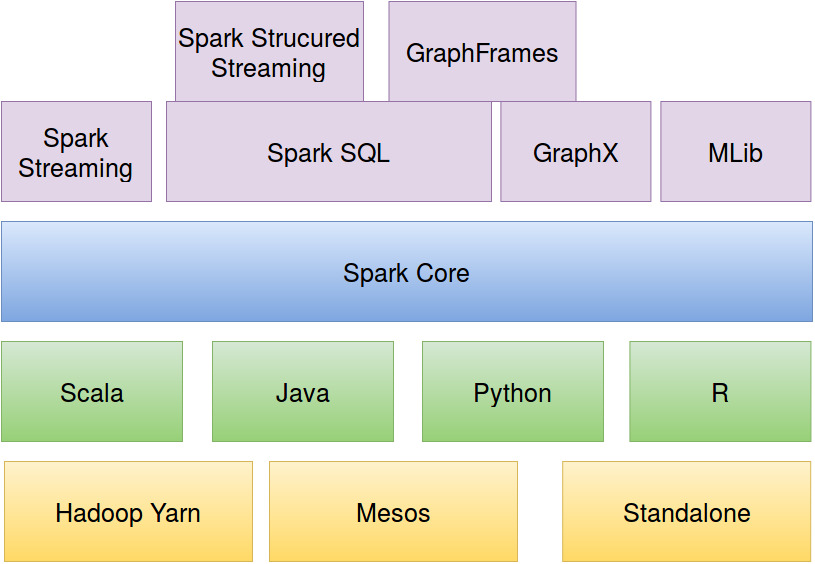
\includegraphics[scale=0.6]{img/componentes}
	\caption{Ecosistema de Spark}
	\label{Ecosistema}
\end{figure}

\section{Spark shell}
Se trata de una consola de lenguaje interactiva con la que poder trabajar de una manera rápida y sencilla con Spark. Está disponible en Scala y Python.\\

\section{Spark UI}
Es una interfaz web con la que podemos monitorizar nuestras aplicaciones en Spark.\\

\vspace*{3.5\baselineskip}
Gracias a todo este ecosistema de librerías y aplicaciones podemos considerar a Spark como una compleja y completa herramienta con la que podemos trabajar en campos muy diversos dentro del Big Data, ofreciendo además versatilidad a la hora de elegir el lenguaje con el que hacerlo.
\chapter{RDD}

Los Resilient Distributed Datasets, RDD, si atendemos a sus siglas, son colecciones de datos distribuidos, de tipado estático, inmutables y de evaluación perezosa usadas por Spark para realizar trabajos cuyo cometido es ir realizando una sucesión de funciones sobre estos RDD con el fin de obtener un resultado.\\
 
Con estas líneas nos pueden asaltar no pocas cuestiones. ¿A qué tipo de colecciones de datos nos referimos? ¿Dónde se distribuyen? ¿Qué quiere decir que son inmutables? ¿Y de evaluación perezosa? Esclarezcamos esta definición de RDD descomponiéndola para asimilar así mejor su contenido:\\
 
Las colecciones de datos que forman los RDD no son solo cualquier tipo de objeto de Python, Java o Scala, sino que  además pueden ser objetos definidos por el usuario. Los datos que conforman el RDD se dividen en particiones que son repartidas entre los diferentes nodos esclavos del clúster. Con inmutables nos referimos a que son solo de lectura, puesto que no se prestan a modificaciones, dado que los RDD van siendo creados a partir de la transformación de otro RDD, de la distribución de una colección de objetos, como puede ser un array, en el driver o de la lectura de datos en memoria, o bien, en algún otro tipo de almacenamiento. Para finalizar este desglose léxico, atendemos al término “evaluación perezosa”. Con él, afirmamos que los RDD son calculados únicamente cuando los datos finales deben computarse, esto es, cuando sobre ellos recae una acción, como veremos más adelante.\\

\section{RDD de pares clave valor}

Son un tipo especial de RDD, compuestos por pares de clave - valor (key-value), lo cual significa que están formados por una lista de tuplas cuyo primer elemento corresponde a la clave y el segundo es el valor que se le asocia a la clave. Podrían ser comparados, pues, con diccionarios o mapas en otros lenguajes de programación, como Python o Java. Spark habilita muchas funciones específicas para trabajar con este tipo de RDDs, ya que le posibilitan actuar en cada clave en paralelo, o reagrupar datos en la red.\\

\section{Propiedades de los RDD}
Ahora que ya hemos estudiado la definición de los RDDs en general, veamos las cinco propiedades internas que caracterizan un RDD en particular: la lista de objetos de partición, la lista con las dependencias de los RDDs padres, una función, una ubicación y el particionador:

\begin{itemize}
\item La lista de objetos de partición que componen el RDD puede ser consultada mediante la función \textit{partitions()}, que devuelve un array con los objetos de partición, que componen las partes del conjunto de datos distribuidos.
 
\item La lista con las dependencias de los RDDs padres, la cual puede ser consultada mediante la función \textit{dependencies()}. Las dependencias pueden ser de dos tipos: narrow o wide. Las primeras corresponden a particiones que dependen de un pequeño subconjunto de particiones del padre, mientras que las segundas son aquellas en las que la partición ha sido creada mediante una reorganización de todos los datos del padre.
 
\item Una función para calcular los elementos de una partición p, dados iteradores para sus particiones padres \textit{iterator(p, parentIters)}. No es común que un usuario llame directamente a esta función. Lo normal es que sea usada por Spark cuando se calculan acciones.
 
\item Una ubicación preferencial de cada partición. Para consultar la localidad de los datos en una partición p podemos usar la función \textit{preferredLocations(p)}, que devuelve una secuencia de string que nos informa sobre cada uno de los nodos donde se almacena la partición p.
 
\item Un particionador. Mediante la función \textit{partitioner()} obtenemos información acerca de si en el  RDD existe una relación entre los datos y la partición asociada a ellos, como un hashPartitioner. \textit{partitioner()} devuelve un optiontype de Scala, siendo None el resultado en aquellos RDD que no sean de tipo Clave Valor.

\end{itemize}

Las tres primeras en conjunto constituyen la ruta desde un RDD hasta su RDD raíz, se conocen como linaje y suponen que cada partición de los datos contenga la información necesaria para ser recalculada, haciendo a Spark tolerante a fallos. Las otras dos son opcionales y se utilizan como optimizadores.\\

\section{Funciones sobre RDDs}
 
Las operaciones que pueden realizarse sobre RDDs se engloban en dos tipos: transformaciones y acciones.\\
 
Las acciones son aquellas operaciones que devuelven algo que no es un RDD. Devuelven información al driver o escriben datos en sistemas de almacenamiento externo. Dado el carácter perezoso de los RDD, son necesarias para la evaluación de un programa de Spark. Algunas acciones mandan la información al driver, por lo que el resultado de cualquier acción debe caber en su memoria. Por este motivo, es preferible evitar acciones que devuelvan el total de los datos al driver, como \textit{collect()}, y usar en su lugar otras que retornen una cantidad elegida por el usuario, como \textit{first()}, \textit{take(n)}, \textit{count}, etcétera.\\
 
Las transformaciones son las operaciones que tienen como resultado un RDD, suponen el concepto básico de trabajo en Spark y constituyen la mayor parte de la potencia de la API de Spark. Dado que  los RDD  son inmutables y están tipados estáticamente, si intentamos realizar una transformación, por pequeña que sea, en un RDD nuestro RDD original no se verá afectado, lo que obtendremos es un nuevo RDD con una nueva definición de sus propiedades. Además, son calculadas de manera perezosa, por lo que su cómputo será ejecutado cuando al RDD resultante se le aplique una acción. Por lo general, las transformaciones tienen un comportamiento a nivel de elemento, actuando de uno en uno de manera paralela en las diferentes particiones de un RDD.\\
 
Las transformaciones se dividen en dos categorías: transformaciones con dependencias \textit{narrow} y transformaciones con dependencias \textit{wide}. Para un buen desarrollo de aplicaciones en Spark, es de vital importancia entender las diferencias entre estas dos categorías, ya que una aplicación construida sin tenerlas en consideración supondrá un impacto muy negativo a nivel de eficiencia.\\
 
Las transformaciones con dependencias \textit{narrow} son aquellas en las que los datos del RDD padre (el RDD sobre el que se aplica la transformación) no necesitan ser mezclados a nivel de partición para calcular el RDD hijo (el RDD resultante de aplicar la transformación al RDD padre), por lo que pueden ser ejecutadas en un subconjunto de datos sin necesidad de información acerca del resto de particiones. De esta manera, el RDD hijo tendrá un número finito de dependencias en las particiones del RDD padre. Transformaciones que se encuentran en esta categoría son \textit{map}, \textit{flatMap}, \textit{filter}.\\
\begin{figure}[H]
	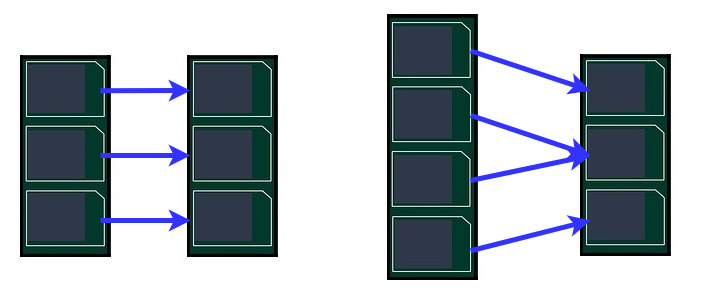
\includegraphics[scale=0.6]{img/narrow}
	\caption{Transformaciones con dependencias narrow}
	\label{foto}
\end{figure}
 
Las transformaciones con dependencias \textit{wide}, por el contrario, son aquellas que requieren un particionado particular de los datos, siendo necesaria la consulta de datos en las distintas particiones del RDD padre, implicando una mezcla en los datos de dichas particiones para computar el RDD hijo; esta operación de compartición de información a través de distintas particiones es conocida en Spark como shuffle, y la estudiaremos detenidamente más adelante. Ejemplos de estas transformaciones son \textit{sort}, \textit{reduceByKey}, \textit{gruoupByKey}.\\
\begin{figure}[H]
	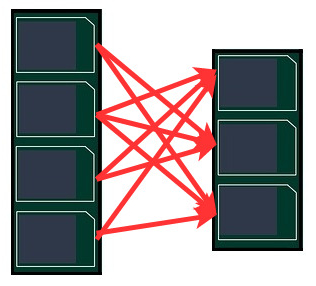
\includegraphics[scale=0.6]{img/wide}
	\centering
	\caption{Transformaciones con dependencias wide}
	\label{foto}
\end{figure}

\section{APIs estructuradas}

Hasta ahora, cuando hemos hablado acerca de las estructuras de datos en Spark lo hemos hecho en términos de RDD. No obstante, hoy por hoy no es la herramienta más utilizada. En este apartado vamos a hablar de los DataFrames y los Datasets, que constituyen las APIs estructuradas de Spark, que son las más usadas en la actualidad.\\

Podemos pensar en los DataFrames y en los Datasets como una tabla distribuida de datos con filas y columnas. El esquema, propiedad inherente a estos, es la lista que define las columnas y los tipos dentro de estas columnas. El usuario puede definirlo, o puede ser leído  por una fuente de datos. Los DataFrames y los Datasets comparten algunas semejanzas con los RDD, como por ejemplo, su inmutabilidad y su evaluación perezosa.\\

\subsection{Datasets}

Están presentes en el ecosistema Spark desde Spark 1.6. Representan conjuntos tipados de datos. En ellos, la comprobación del tipado se realiza en tiempo de compilación. Sólo están disponibles para los lenguajes basados en JVM, es decir, para Scala y para Java, dado que los tipos que admite son los tipos de Java o case class de Scala.\\

\subsection{Los DataFrames} 

Se trata de la API estructurada más usada actualmente y aparecieron en la versión Spark 1.3. Se suele decir que se trata de conjuntos no tipados, lo cual es incorrecto. La comprobación del tipado especificado se realiza en tiempo de ejecución. Internamente, Spark trata a los DataFrames como Datasets de tipo \textit{row}, que permite liberarse de los costes de recolección de basura y creación de instancias de objetos que implican los tipos de JVM. Están disponibles en cuatro lenguajes: Java, Python, Scala y R. 



\chapter{Arquitectura de Spark}

El término “arquitectura” en informática remite a la estructura lógica y física de los componentes de una computadora. Si nos detenemos a estudiar la arquitectura de Spark, la primera característica identificativa es su uso de la conocida arquitectura maestro-esclavo o maestro-trabajador, que, como bien indica su terminología, consta de un nodo maestro y muchos nodos esclavos.\\
 
La arquitectura de Spark se compone de dos procesos: el driver y los executors. Ambos serán descritos más adelante, pero aclaremos por ahora que el driver es el coordinador central, el cual se comunica con el cluster manager, encargado de orquestar los nodos esclavos, donde corren los executors y que, además, el driver y los executors se ejecutan en sus propios procesos de Java.\\
 
Para ir dibujando nuestra arquitectura necesitamos preguntarnos cómo se ponen en funcionamiento las aplicaciones en Spark. El proceso es el siguiente: Las aplicaciones de Spark se ejecutan como conjuntos de procesos independientes en un clúster, coordinados por el objeto SparkContext en su programa principal, el driver. Cuando ejecutamos Spark en un clúster, SparkContext se conecta al cluster manager, encargado de asignar recursos en el clúster. Una vez conectado, Spark adquiere executors en los nodos del clúster, que son procesos que ejecutan cúlculos y almacenan datos para su aplicación. A continuación, envía su código de aplicación (definido por archivos JAR o Python pasados a SparkContext) a los esclavos. Por último, SparkContext envía tareas a los esclavos para que se ejecuten.\\
 
Spark puede ejecutar varias aplicaciones en un clúster al mismo tiempo. Las aplicaciones están programadas por el administrador del clúster (cluster manager) y corresponden a un SparkContext. Cada aplicación obtiene sus propios agentes executors, que permanecen activos durante toda la aplicación y ejecutan tareas en varios subprocesos. Este hecho tiene la ventaja de aislar aplicaciones entre sí, tanto en el lado de la programación (cada driver programa sus propias tareas), como en el lado del executor (las tareas de diferentes aplicaciones se ejecutan en diferentes Máquinas Virtuales Java). Sin embargo, también significa que los datos no se pueden compartir en diferentes aplicaciones Spark sin escribirlo en un sistema de almacenamiento externo.\\
 
\section{Driver}
 
Como hemos señalado antes, el driver es el coordinador central, ya que un programa Spark se ejecuta en el nodo del driver y este envía instrucciones a los executors. Es un proceso JVM que ejecuta la función main() de la aplicación y crea el SparkContext para una aplicación de Spark. También aloja el DAG Scheduler y el Task Scheduler, de los que hablaremos no muy tarde.\\

El driver debe ser direccionable a través de la red desde los nodos esclavos, en tanto que es el que escucha y acepta las conexiones entrantes de sus executors a lo largo de su vida útil. Además, el driver es el encargado de traducir el código de usuario en un trabajo específico y de crear tareas convirtiendo aplicaciones en pequeñas unidades de ejecución.\\
 
\section{Executors}
 
Son agentes distribuidos responsables de la ejecución de las tareas, siendo ellos los que procesan los datos, los mantienen en memoria o los almacenan en disco.\\
 
Cada aplicación tiene sus propios executors. Los executor se ejecutan durante toda la vida de una aplicación de Spark. Pueden ejecutar múltiples tareas a lo largo de su vida, tanto de forma secuencial como paralela. Suelen ser de asignación estática. No obstante, en caso de que así lo requiramos, podemos configurarlos para hacer la asignación dinámica.\\
 
También informan de las métricas parciales mediante el uso del hilo del transmisor Heartbeat. Cuando un executor se inicia, se registra con el driver, comunicándose directamente con él para ejecutar tareas.\\
 
Sobre la ubicación de los executor, cabe señalar que residen en los nodos esclavos del clúster, que son cualquier nodo que pueda ejecutar código de aplicación en el clúster. Cada executor es su propia JVM, y un executor no puede abarcar múltiples nodos, aunque un nodo puede contener varios executors.\\
 
% AÑADIR NOTA A PIE DE PÁGINA ACERCA DE QUÉ SON LOS AGENTES
 
\section{SparkContext}
 
El SparkContext es una variable de entorno que configura los servicios internos y establece una conexión con un entorno de ejecución de Spark. Es decir, con el clúster.
Una vez que se crea un SparkContext, puede usarlo para crear RDD, acumuladores y variables broadcast, acceder a los servicios de Spark y ejecutar trabajos (hasta que se detenga SparkContext). Proporciona acceso al clúster a través del cluster manager.
SparkContext es esencialmente un cliente del entorno de ejecución de Spark y actúa como el maestro de su aplicación.\\

SparkContext determina cuántos recursos se asignan a cada executor. Como veremos más adelante, cuando se lanza un trabajo de Spark, cada executor tiene ranuras (slots) para ejecutar las tareas necesarias para calcular un RDD. De esta forma, podemos pensar en un SparkContext como un conjunto de parámetros de configuración para ejecutar trabajos de Spark. Estos parámetros (por ejemplo, la URL del nodo maestro) están expuestos en el objeto SparkConf, utilizado para crear un SparkContext.\\
 
\section{DAG Sheduler}
 
El DAGSheduler, a quien ya habíamos introducido, es el responsable de manejar la ejecución de una aplicación en Spark, dividiéndola en trabajos, etapas y tareas. Estos conceptos los estudiaremos detenidamente más adelante para así centrarnos a lo largo de este subapartado en comprender cómo actúa el DAGScheduler de Spark y por qué este comportamiento supone una mejora con respecto a otros sistemas.\\

Se trata de la capa de planificación de alto nivel \cite{05GitDAG} que implementa la programación orientada a la etapa. Lo hace calculando un DAG (directed aciclid graph) de etapas para cada trabajo, realizando un seguimiento de los RDD, a la par que busca un cronograma mínimo para ejecutar el trabajo. Por lo tanto, es el encargado de transformar un plan de ejecución lógico (es decir, el linaje de RDD de dependencias) en un plan de ejecución físico. Además de crear un DAG de etapas, DAGScheduler determina las ubicaciones más apropiadas para ejecutar cada tarea, teniendo en cuenta el estado actual de la memoria caché, evitando así recalcular RDD que hayan sido cacheados. También se ocupa de borrar las estructuras de datos una vez hayan finalizado las tareas que dependen de ellos, optimizando así el uso de memoria. Por último, bajo su responsabilidad está la recuperación ante fallas debidas a la pérdida de archivos durante el shuffle. Lo hace volviendo a computar las etapas afectadas en las particiones perdidas.\\

Este modelo es una generalización del modelo MapReduce, el cual crea un DAG con dos estados, Map y Reduce. El cambio de etapas en un DAG en Spark viene marcado por una transformación con dependencias wide, por lo tanto, puede canalizar transformaciones con dependencias narrow juntas, sin necesidad de escribir a disco entre cada una, obteniendo así un mejor rendimiento que el de MapReduce, que necesita escribir en disco los resultados entre las etapas Map y Reduce.\\

\begin{figure}[H]
	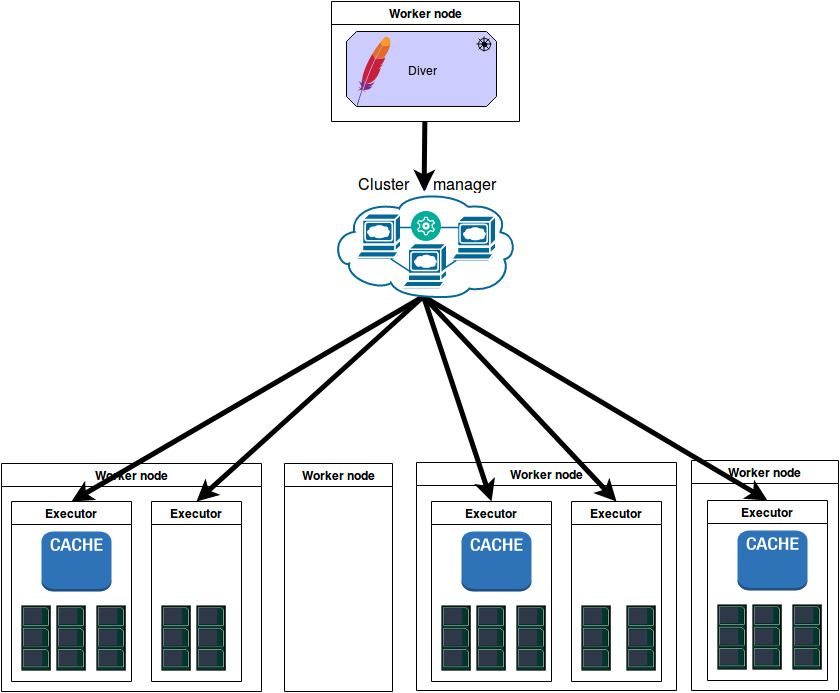
\includegraphics[scale=0.6]{img/arquitectura}
	\centering
	\caption{Arquitectura de Spark}
	\label{Arquitectura}
\end{figure}

\chapter{Cómo opera Spark}

En este apartado vamos a tratar qué sucede internamente cuando estamos trabajando con Spark. Para iniciarnos en dicha materia debemos familiarizarnos antes con algunos conceptos propios de Spark.

\section{Tareas}
Las tareas son unidades de trabajo individuales , cada una enviada a una máquina, es decir, una tarea no se puede ejecutar en más de un executor, cada tarea atacará a una partición específica de los datos. Dicho de otra manera, una tarea es simplemente una unidad de cálculo aplicada a una unidad de datos (partición). Particionar los RDD en un mayor número de particiones significa que se pueden ejecutar más en paralelo, siempre y cuando el clúster tenga recursos suficientes. Spark no puede ejecutar más tareas a la vez que el número de núcleos por executor por la cantidad de executors.El número de tareas por etapa corresponde al número de particiones en el RDD de salida de esa etapa.\\

Cada tarea realiza internamente los mismos pasos:\\

\begin{enumerate}

\item Obtener su entrada, ya sea desde el almacenamiento de datos (si el RDD es un RDD de entrada), un RDD existente (para datos ya almacenados en caché), o salidas de shuffle.\\

\item Realizar la operación necesaria para calcular los RDDs que representa.\\

\item Escribirá la salida de shuffle, en almacenamiento externo o de vuelta al driver (si es el RDD final de una acción como \textit{count()}).
\end{enumerate}

El conjunto de tareas producidas por una transformación con dependencias \textit{narrow} se denomina etapa.\\

\section{Etapas}
Para ser más eficiente, Spark agrupa las operaciones que pueden ser aplicadas en una sola partición, y, consecuentemente, en una única máquina sin que sea necesaria comunicación en red entre los nodos esclavos, esto es, cuando no se requiere información de otras máquinas. Es decir, canaliza juntas las transformaciones con dependencias \textit{narrow}, mientras que las transformaciones con dependencias \textit{wide} suponen el límite entre una etapa y otra.\\

En consecuencia, entre una etapa y el siguiente se necesita comunicación con el driver, por lo que se han de ejecutar en secuencia. Sin embargo, en casos donde no se requiera información de otra etapa, por ejemplo, aplicar operaciones a dos RDD sin ningún padre común, se pueden calcular en paralelo.\\

\begin{figure}[H]
	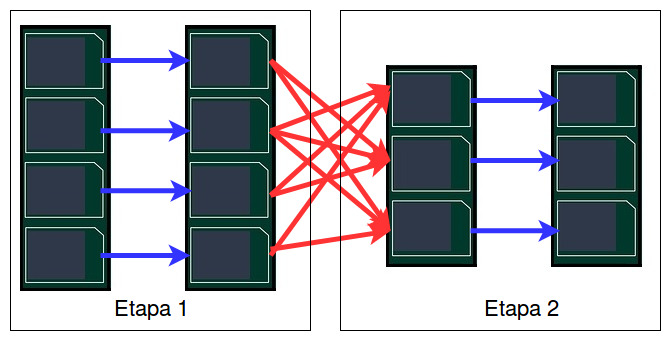
\includegraphics[scale=0.6]{img/etapas} 
	\centering
	\caption{pie de foto}
	\label{foto}
\end{figure}

Podemos clasificar las etapas en dos categorías diferentes, según lo que marque su final:\\

\begin{itemize}
\item ShuffleMapStage, que escribe los archivos de salida de shuffle.
\item ResultStage, para la etapa final que ejecuta una acción.
\end{itemize}

Las agrupaciones de etapas fruto de una acción se conocen como trabajo. Las etapas suelen compartirse en varios trabajos, si estos trabajos reutilizan los mismos RDD.\\

\section{Trabajo}
Suponen el elemento más alto de la jerarquía de ejecución de Spark. Cada trabajo de Spark corresponde a una acción, y suponen el desencadenante para comenzar el cómputo sobre los RDD, debido al carácter perezoso de estos. \\

\section{Aplicación}
Por último, definimos a cada uno de los programas en los que se crea un SparkContext como una aplicación de Spark. Entre diferentes aplicaciones no se comparte memoria ni recursos.\\

Ahora que ya conocemos las distintas fases por las que pasa toda aplicación de Spark, falta por abordar una cuestión. Como hemos visto, la memoria entre etapas no puede ser compartida por no estar en la misma máquina virtual, por lo que nos surge la pregunta de cómo compartir información entre etapas. La respuesta sería escribiendo a disco, operación conocida como shuffle.\\

\section{Shuffle}
Según la documentación oficial de Spark, el shuffle es “el mecanismo de Spark para redistribuir los datos de manera que se agrupen de manera diferente en las particiones”. Es conveniente aclarar que no todo movimiento de datos por el clúster es considerado como shuffle. Las acciones, escrituras o lecturas de una fuente externa no se consideran shuffle. La fase de shuffle representa una repartición física de los datos, esto es, conlleva escritura en disco. Esto contradice la definición inicial que dimos de Spark como  motor de computación en memoria, pero se trata de momentos concretos en los que debido a una transformación con dependencias \textit{wide}, es decir, cuando necesite combinar los datos de distintas etapas, o por saturación de memoria, en vez de mantener los datos cacheados los escribe temporalmente a disco, tras lo cual se genera una nueva etapa con un nuevo conjunto de particiones.\\

Su comportamiento varía dependiendo del Shuffle Manager que usemos y cada uno tendrá su Caso de Uso. Tratar los diferentes shuffle manager va más allá de lo que pretendemos abordar en este texto, por lo que únicamente nos centraremos en las propiedades generales.\\

Operaciones que pueden causar shuffle son aquellas que implican una repartición de los datos entre particiones, como repartition y coalesce, operaciones \textit{ByKey}, excepto  \textit{countByKey} y operaciones de mezcla de RDDs como \textit{cogroup} y \textit{join}.\\

Se trata de una operación muy costosa, pues debe leer todas las particiones para encontrar todos los valores de todas las claves, y luego unir los valores de las particiones para calcular el resultado final de cada valor, esto conlleva escritura y lectura en disco, serialización de datos y movimiento de entrada y salida por la red \cite{6RDD_Documentation}.\\

La fase de shuffle se desarrolla en dos partes: map y reduce. En la parte de map, Spark genera archivos intermedios que son escritos en disco en la ruta local de cada nodo. Estos archivos son conservados hasta que los RDD a los que corresponden ya no se utilizan, de esta manera, en caso de fallo no es necesario que vuelvan a ser calculados. Cada tarea map escribe un archivo por cada tarea Reduce. El directorio de almacenamiento temporal en disco puede ser configurado en la propiedad spark.local.dir que se configura a nivel de application. Además, spark brinda la opción de comprimir los archivos de salida Map, especificados por el parámetro \textit{spark.shuffle.compress}.\\

Un efecto de lado provocado por esta persistencia en disco durante la fase de shuffle es que la ejecución de un nuevo trabajo sobre los datos que ya se han pasado por la fase shuffle no vuelve a ejecutar la parte map del shuffle. Debido a que los archivos shuffle ya se habían escrito anteriormente en disco, Spark sabe que puede usarlos para ejecutar únicamente la parte reduce del shuffle. Pese a esta optimización automática,  para un mejor rendimiento es preferible realizar su propio almacenamiento en caché con el método caché, que le permite controlar exactamente qué datos guardar y dónde.\\

Durante la fase de reduce, Spark requiere que todos los datos quepan en memoria. Cuando la memoria requerida de cada tarea reduce excede la asignada, se emite una excepción de falta de memoria y se debe interrumpir todo el trabajo. Para evitar quedarse sin memoria, se debe especificar un valor suficientemente alto para la cantidad de tareas reduce.\\

Llegados a este punto ya estamos en disposición de poder analizar qué sucede internamente durante una aplicación de Spark:\\

El código escrito por un usuario define un DAG de RDD. En primer lugar, Spark comprueba si el código escrito por el usuario es válido. Tras esto, Spark lo convierte en un flujo lógico de operaciones, el plan lógico \cite{6DAGandPE} (también conocido como DAG de dependencias). Cuando se realiza una acción este plan lógico se pasa a través de SparkContext al DAG Scheduler, que lo usa para crear un plan de ejecución físico, el DAG de etapas, que consiste en tareas agrupadas en etapas, las cuales son enviadas como TaskSets a una implementación TasScheduler subyacente, que es el encargado de enviar las tareas para su ejecución en el clúster a través del cluster manager \cite{6DFariDAG}. En este punto Spark ejecuta este plan en el clúster.\\

Spark cuenta con mecanismos internos para optimizar tanto el plan lógico como el plan físico, y también realiza optimizaciones en tiempo de ejecución. Estos difieren en función de si estamos tratando con las APIs estructuradas o con RDDs. En cualquier caso, el plan físico siempre es ejecutado sobre RDDs.

\chapter{Codigo}

\chapter{Conclusiones}

\addcontentsline{toc}{chapter}{Referencias}
\bibliographystyle{unsrt} %abbry unsrt
\bibliography{capitulos/bibliografia}

\end{document}






































